\documentclass[tikz, border=12pt]{standalone}
\usepackage[utf8]{inputenc}
\usepackage{amsmath,amssymb}
\usepackage{tikz}
\usetikzlibrary{shapes.geometric, arrows.meta, positioning, calc, backgrounds, fit, decorations.pathreplacing}

% ==============================================================================
% Color Palette: IEEE Transactions Professional Palette
% ==============================================================================
\definecolor{pebg}{RGB}{248, 250, 252}         % Soft slate white for PE fill
\definecolor{peborder}{RGB}{71, 85, 105}       % Slate gray border
\definecolor{actcolor}{RGB}{30, 64, 175}       % Deep Sapphire Blue (Activation path)
\definecolor{actbg}{RGB}{239, 246, 255}
\definecolor{weightcolor}{RGB}{4, 120, 87}     % Forest Emerald Green (Weight path)
\definecolor{weightbg}{RGB}{236, 253, 245}
\definecolor{acccolor}{RGB}{180, 83, 9}        % Warm Amber / Ochre (Accumulator path)
\definecolor{accbg}{RGB}{254, 243, 199}
\definecolor{ctrlcolor}{RGB}{185, 28, 28}      % Dark Crimson (Control signals)
\definecolor{ctrlbg}{RGB}{254, 242, 242}
\definecolor{regcolor}{RGB}{224, 231, 255}     % Register fill
\definecolor{regborder}{RGB}{67, 56, 202}
\definecolor{buscolor}{RGB}{30, 41, 59}        % Dark charcoal for buses

\begin{document}
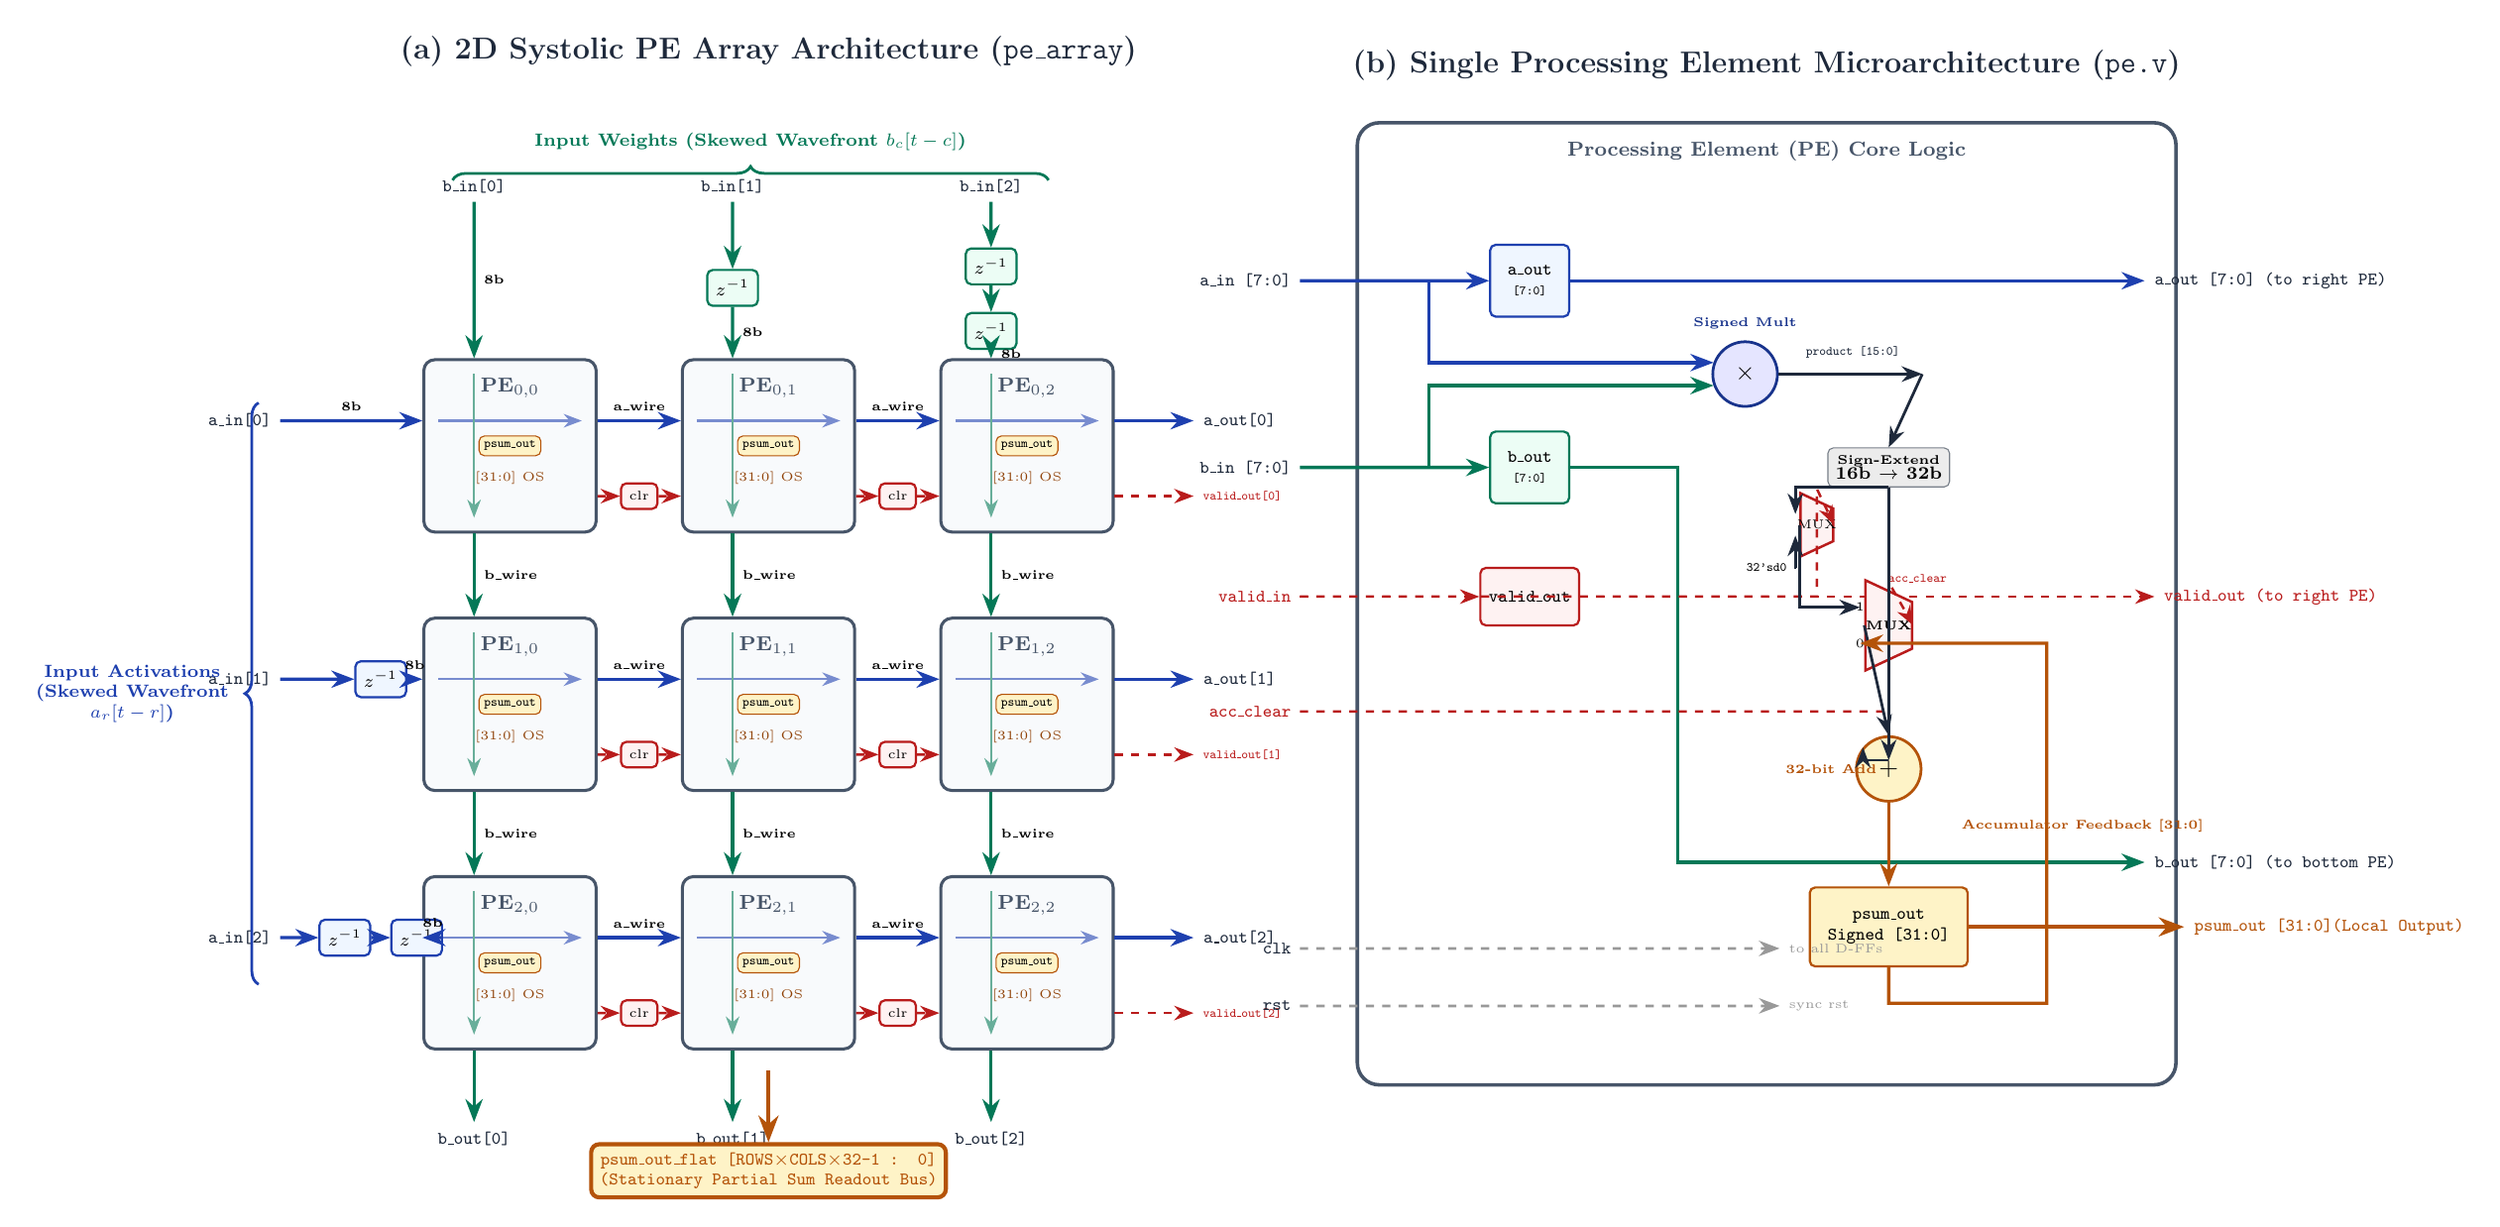
\begin{tikzpicture}[
    scale=0.92, every node/.style={transform shape},
    >=Stealth,
    % Node styles
    pe_box/.style={draw=peborder, fill=pebg, rounded corners=4pt, line width=1.1pt, minimum width=2.4cm, minimum height=2.4cm, align=center},
    reg_dff/.style={draw=regborder, fill=regcolor, line width=0.8pt, rounded corners=2pt, minimum width=1.1cm, minimum height=0.65cm, align=center, font=\scriptsize\bfseries\ttfamily},
    arith_op/.style={draw=acccolor, fill=accbg, line width=1.0pt, circle, minimum size=0.9cm, align=center, font=\normalsize\bfseries},
    mux_block/.style={trapezium, draw=ctrlcolor, fill=ctrlbg, line width=0.9pt, trapezium angle=65, minimum width=1.2cm, minimum height=0.65cm, rotate=-90, align=center, font=\tiny\bfseries},
    port_text/.style={font=\scriptsize\bfseries\ttfamily, color=buscolor},
    label_subfig/.style={font=\large\bfseries, color=buscolor},
    label_title/.style={font=\small\bfseries, color=buscolor},
    bus_arrow/.style={draw=buscolor, line width=1.0pt, ->},
    act_arrow/.style={draw=actcolor, line width=1.2pt, ->},
    weight_arrow/.style={draw=weightcolor, line width=1.2pt, ->},
    ctrl_arrow/.style={draw=ctrlcolor, line width=0.9pt, dashed, ->},
    acc_arrow/.style={draw=acccolor, line width=1.2pt, ->}
]

    % ==========================================================================
    % SUBFIGURE (a): 2D OUTPUT-STATIONARY SYSTOLIC PE ARRAY (pe_array)
    % ==========================================================================
    \begin{scope}[local bounding box=mesh_array]
        
        % Subfigure Title
        \node[label_subfig] at (3.6, 5.5) {(a) 2D Systolic PE Array Architecture (\texttt{pe\_array})};

        % Generate 3x3 PE Grid
        \foreach \r in {0, 1, 2} {
            \foreach \c in {0, 1, 2} {
                \node[pe_box] (PE_\r_\c) at (\c*3.6, -\r*3.6) {};
                
                % PE Inner Details
                \node[font=\footnotesize\bfseries, color=peborder] at (\c*3.6, -\r*3.6 + 0.8) {PE$_{\r,\c}$};
                \node[draw=acccolor, fill=accbg, rounded corners=2pt, font=\tiny\ttfamily\bfseries, inner sep=2pt] 
                    at (\c*3.6, -\r*3.6) {psum\_out};
                \node[font=\tiny, color=acccolor!80!black] at (\c*3.6, -\r*3.6 - 0.45) {[31:0] OS};

                % Horizontal forward internal indicator
                \draw[actcolor!60, line width=0.8pt, ->] (\c*3.6 - 1.0, -\r*3.6 + 0.35) -- (\c*3.6 + 1.0, -\r*3.6 + 0.35);
                % Vertical forward internal indicator
                \draw[weightcolor!60, line width=0.8pt, ->] (\c*3.6 - 0.5, -\r*3.6 + 1.0) -- (\c*3.6 - 0.5, -\r*3.6 - 1.0);
            }
        }

        % --- ACTIVATION INPUTS & SKEW REGISTERS (LEFT BOUNDARY) ---
        % Row 0: no skew
        \node[port_text, anchor=east] (a_in_0) at (-3.2, 0.35) {a\_in[0]};
        \draw[act_arrow] (a_in_0) -- node[above, font=\tiny\bfseries] {8b} ([yshift=0.35cm]PE_0_0.west);

        % Row 1: 1 skew register (D)
        \node[port_text, anchor=east] (a_in_1) at (-3.2, -3.6 + 0.35) {a\_in[1]};
        \node[reg_dff, fill=actbg, draw=actcolor, minimum width=0.6cm, minimum height=0.5cm] (skew_a1) at (-1.8, -3.6 + 0.35) {$z^{-1}$};
        \draw[act_arrow] (a_in_1) -- (skew_a1);
        \draw[act_arrow] (skew_a1) -- node[above, font=\tiny\bfseries] {8b} ([yshift=0.35cm]PE_1_0.west);

        % Row 2: 2 skew registers (D D)
        \node[port_text, anchor=east] (a_in_2) at (-3.2, -7.2 + 0.35) {a\_in[2]};
        \node[reg_dff, fill=actbg, draw=actcolor, minimum width=0.6cm, minimum height=0.5cm] (skew_a2_1) at (-2.3, -7.2 + 0.35) {$z^{-1}$};
        \node[reg_dff, fill=actbg, draw=actcolor, minimum width=0.6cm, minimum height=0.5cm] (skew_a2_2) at (-1.3, -7.2 + 0.35) {$z^{-1}$};
        \draw[act_arrow] (a_in_2) -- (skew_a2_1);
        \draw[act_arrow] (skew_a2_1) -- (skew_a2_2);
        \draw[act_arrow] (skew_a2_2) -- node[above, font=\tiny\bfseries] {8b} ([yshift=0.35cm]PE_2_0.west);

        % Activation Wavefront Brace
        \draw[decorate, decoration={brace, amplitude=5pt, mirror}, color=actcolor, line width=1pt]
            (-3.5, 0.6) -- (-3.5, -7.5) node[midway, left=8pt, font=\scriptsize\bfseries, align=center, color=actcolor] 
            {Input Activations\\(Skewed Wavefront\\$a_{r}[t-r]$)};

        % --- WEIGHT INPUTS & SKEW REGISTERS (TOP BOUNDARY) ---
        % Col 0: no skew
        \node[port_text, anchor=south] (b_in_0) at (-0.5, 3.4) {b\_in[0]};
        \draw[weight_arrow] (b_in_0) -- node[right, font=\tiny\bfseries] {8b} ([xshift=-0.5cm]PE_0_0.north);

        % Col 1: 1 skew register (D)
        \node[port_text, anchor=south] (b_in_1) at (3.6 - 0.5, 3.4) {b\_in[1]};
        \node[reg_dff, fill=weightbg, draw=weightcolor, minimum width=0.6cm, minimum height=0.5cm] (skew_b1) at (3.6 - 0.5, 2.2) {$z^{-1}$};
        \draw[weight_arrow] (b_in_1) -- (skew_b1);
        \draw[weight_arrow] (skew_b1) -- node[right, font=\tiny\bfseries] {8b} ([xshift=-0.5cm]PE_0_1.north);

        % Col 2: 2 skew registers (D D)
        \node[port_text, anchor=south] (b_in_2) at (7.2 - 0.5, 3.4) {b\_in[2]};
        \node[reg_dff, fill=weightbg, draw=weightcolor, minimum width=0.6cm, minimum height=0.5cm] (skew_b2_1) at (7.2 - 0.5, 2.5) {$z^{-1}$};
        \node[reg_dff, fill=weightbg, draw=weightcolor, minimum width=0.6cm, minimum height=0.5cm] (skew_b2_2) at (7.2 - 0.5, 1.6) {$z^{-1}$};
        \draw[weight_arrow] (b_in_2) -- (skew_b2_1);
        \draw[weight_arrow] (skew_b2_1) -- (skew_b2_2);
        \draw[weight_arrow] (skew_b2_2) -- node[right, font=\tiny\bfseries] {8b} ([xshift=-0.5cm]PE_0_2.north);

        % Weight Wavefront Brace
        \draw[decorate, decoration={brace, amplitude=5pt}, color=weightcolor, line width=1pt]
            (-0.8, 3.7) -- (7.5, 3.7) node[midway, above=8pt, font=\scriptsize\bfseries, align=center, color=weightcolor] 
            {Input Weights (Skewed Wavefront $b_{c}[t-c]$)};

        % --- HORIZONTAL & VERTICAL INTERCONNECTS BETWEEN PEs ---
        \foreach \r in {0, 1, 2} {
            % Horiz 0 -> 1
            \draw[act_arrow] ([yshift=0.35cm]PE_\r_0.east) -- node[above, font=\tiny\bfseries] {a\_wire} ([yshift=0.35cm]PE_\r_1.west);
            % Horiz 1 -> 2
            \draw[act_arrow] ([yshift=0.35cm]PE_\r_1.east) -- node[above, font=\tiny\bfseries] {a\_wire} ([yshift=0.35cm]PE_\r_2.west);
            % Horiz Out
            \draw[act_arrow] ([yshift=0.35cm]PE_\r_2.east) -- ++(1.1, 0) node[port_text, anchor=west] {a\_out[\r]};

            % Valid / Clear horizontal pipeline
            \node[reg_dff, fill=ctrlbg, draw=ctrlcolor, minimum width=0.5cm, minimum height=0.35cm, font=\tiny] (clr_r_\r_0) at (1.8, -\r*3.6 - 0.7) {clr};
            \draw[ctrl_arrow] ([yshift=-0.7cm]PE_\r_0.east) -- (clr_r_\r_0);
            \draw[ctrl_arrow] (clr_r_\r_0) -- ([yshift=-0.7cm]PE_\r_1.west);

            \node[reg_dff, fill=ctrlbg, draw=ctrlcolor, minimum width=0.5cm, minimum height=0.35cm, font=\tiny] (clr_r_\r_1) at (5.4, -\r*3.6 - 0.7) {clr};
            \draw[ctrl_arrow] ([yshift=-0.7cm]PE_\r_1.east) -- (clr_r_\r_1);
            \draw[ctrl_arrow] (clr_r_\r_1) -- ([yshift=-0.7cm]PE_\r_2.west);

            \draw[ctrl_arrow] ([yshift=-0.7cm]PE_\r_2.east) -- ++(1.1, 0) node[font=\tiny\bfseries\ttfamily, color=ctrlcolor, anchor=west] {valid\_out[\r]};
        }

        \foreach \c in {0, 1, 2} {
            % Vert 0 -> 1
            \draw[weight_arrow] ([xshift=-0.5cm]PE_0_\c.south) -- node[right, font=\tiny\bfseries] {b\_wire} ([xshift=-0.5cm]PE_1_\c.north);
            % Vert 1 -> 2
            \draw[weight_arrow] ([xshift=-0.5cm]PE_1_\c.south) -- node[right, font=\tiny\bfseries] {b\_wire} ([xshift=-0.5cm]PE_2_\c.north);
            % Vert Out
            \draw[weight_arrow] ([xshift=-0.5cm]PE_2_\c.south) -- ++(0, -1.0) node[port_text, anchor=north] {b\_out[\c]};
        }

        % Global Output Flat Bus Indicator
        \draw[bus_arrow, line width=1.5pt, acccolor] (3.6, -8.7) -- ++(0, -1.0) 
            node[draw=acccolor, fill=accbg, rounded corners=3pt, font=\scriptsize\bfseries\ttfamily, align=center, anchor=north] 
            {psum\_out\_flat [ROWS$\times$COLS$\times$32-1 : 0]\\(Stationary Partial Sum Readout Bus)};

    \end{scope}

    % ==========================================================================
    % SUBFIGURE (b): INTERNAL PROCESSING ELEMENT MICROARCHITECTURE (pe.v)
    % ==========================================================================
    \begin{scope}[shift={(14.0, -2.5)}, local bounding box=pe_micro]
        
        % Subfigure Title
        \node[label_subfig] at (3.5, 7.8) {(b) Single Processing Element Microarchitecture (\texttt{pe.v})};

        % PE Outer Boundary Box
        \draw[draw=peborder, fill=white, rounded corners=8pt, line width=1.3pt] (-2.2, -6.4) rectangle (9.2, 7.0);
        \node[font=\footnotesize\bfseries, color=peborder] at (3.5, 6.6) {Processing Element (PE) Core Logic};

        % --- INPUT PORTS (LEFT) ---
        \node[port_text, anchor=east] (p_ain)   at (-3.0, 4.8) {a\_in [7:0]};
        \node[port_text, anchor=east] (p_bin)   at (-3.0, 2.2) {b\_in [7:0]};
        \node[port_text, color=ctrlcolor, anchor=east] (p_vin)   at (-3.0, 0.4) {valid\_in};
        \node[port_text, color=ctrlcolor, anchor=east] (p_clr)   at (-3.0, -1.2) {acc\_clear};
        \node[port_text, anchor=east] (p_clk)   at (-3.0, -4.5) {clk};
        \node[port_text, anchor=east] (p_rst)   at (-3.0, -5.3) {rst};

        % --- FORWARDING REGISTERS (D-FF) ---
        % a_out register
        \node[reg_dff, fill=actbg, draw=actcolor, minimum height=1.0cm] (r_aout) at (0.2, 4.8) {a\_out\\{\tiny [7:0]}};
        % b_out register
        \node[reg_dff, fill=weightbg, draw=weightcolor, minimum height=1.0cm] (r_bout) at (0.2, 2.2) {b\_out\\{\tiny [7:0]}};
        % valid_out register
        \node[reg_dff, fill=ctrlbg, draw=ctrlcolor, minimum height=0.8cm] (r_vout) at (0.2, 0.4) {valid\_out};

        % Forwarding connection to outputs
        \draw[act_arrow] (p_ain) -- (r_aout.west);
        \draw[act_arrow] (r_aout.east) -- ++(8.0, 0) node[port_text, anchor=west] {a\_out [7:0] (to right PE)};

        \draw[weight_arrow] (p_bin) -- (r_bout.west);
        \draw[weight_arrow] (r_bout.east) -- ++(1.5, 0) -- ++(0, -5.5) -- ++(6.5, 0) node[port_text, anchor=west] {b\_out [7:0] (to bottom PE)};

        \draw[ctrl_arrow] (p_vin) -- (r_vout.west);
        \draw[ctrl_arrow] (r_vout.east) -- ++(8.0, 0) node[port_text, color=ctrlcolor, anchor=west] {valid\_out (to right PE)};

        % --- SIGNED MULTIPLIER (INT8 x INT8 -> INT16) ---
        \node[arith_op, draw=actcolor!80!black, fill=blue!10] (mult) at (3.2, 3.5) {$\mathbf{\times}$};
        \node[font=\tiny\bfseries, color=actcolor!80!black] at (3.2, 4.2) {Signed Mult};

        \draw[act_arrow] (-1.2, 4.8) |- (mult.160);
        \draw[weight_arrow] (-1.2, 2.2) |- (mult.200);

        % Product wire
        \node[font=\tiny\ttfamily\bfseries, color=buscolor] at (4.7, 3.8) {product [15:0]};
        \draw[bus_arrow] (mult.east) -- ++(2.0, 0) coordinate (prod_pt);

        % --- SIGN EXTENSION BLOCK (16b -> 32b) ---
        \node[draw=buscolor!60, fill=gray!15, rounded corners=2pt, font=\tiny\bfseries, align=center, inner sep=3pt] 
            (sext) at (5.2, 2.2) {Sign-Extend\\{\scriptsize 16b $\rightarrow$ 32b}};
        \draw[bus_arrow] (prod_pt) -- (sext.north);

        % --- MULTIPLEXING LOGIC (acc_clear & valid_in) ---
        % Mux Clear
        \node[mux_block] (mux_clr) at (5.2, 0.0) {};
        \node[font=\tiny\bfseries, rotate=0] at (5.2, 0.0) {MUX};
        \node[font=\tiny] at (4.8, 0.25) {1};
        \node[font=\tiny] at (4.8, -0.25) {0};

        % Zero constant node
        \node[font=\tiny\ttfamily] (c_zero) at (3.5, 0.8) {32'sd0};

        % Mux for valid_in condition during clear
        \node[mux_block, scale=0.7] (mux_vinit) at (4.2, 1.4) {};
        \node[font=\tiny] at (4.2, 1.4) {\tiny MUX};
        \draw[ctrl_arrow] (p_vin) -| (4.2, 1.9) -- (mux_vinit.north);
        \draw[bus_arrow] (sext.south) -| (3.9, 1.55);
        \draw[bus_arrow] (c_zero) -| (3.9, 1.25);
        \draw[bus_arrow] (mux_vinit.south) |- (4.8, 0.25);

        % Control input acc_clear to Mux Clear
        \draw[ctrl_arrow] (p_clr) -| (5.2, 0.6) -- (mux_clr.north);
        \node[font=\tiny\ttfamily\bfseries, color=ctrlcolor] at (5.6, 0.65) {acc\_clear};

        % --- SIGNED 32-BIT ACCUMULATOR ADDER ---
        \node[arith_op, draw=acccolor, fill=accbg] (adder) at (5.2, -2.0) {$\mathbf{+}$};
        \node[font=\tiny\bfseries, color=acccolor] at (4.4, -2.0) {32-bit Add};

        \draw[bus_arrow] (sext.south) -- ++(0, -3.8) coordinate (add_in2);
        \draw[bus_arrow] (add_in2) -| (adder.140);
        \draw[bus_arrow] (mux_clr.south) -- (adder.north);

        % --- ACCUMULATOR REGISTER (psum_out) ---
        \node[reg_dff, fill=accbg, draw=acccolor, minimum width=2.2cm, minimum height=1.1cm] (r_psum) at (5.2, -4.2) {
            psum\_out\\{\scriptsize Signed [31:0]}
        };

        % Output to adder
        \draw[acc_arrow] (adder.south) -- (r_psum.north);

        % Feedback loop
        \draw[acc_arrow] (r_psum.south) -- ++(0, -0.5) -- ++(2.2, 0) coordinate (fb_turn) 
            -- ([yshift=-0.25cm]fb_turn |- mux_clr.center) -- (4.8, -0.25);
        \node[font=\tiny\bfseries, color=acccolor] at (7.9, -2.8) {Accumulator Feedback [31:0]};

        % Output Port
        \draw[acc_arrow, line width=1.4pt] (r_psum.east) -- ++(3.0, 0) 
            node[port_text, color=acccolor, anchor=west] {psum\_out [31:0]\\(Local Output)};

        % Clock & Reset routing
        \draw[bus_arrow, dashed, color=gray!80] (p_clk) -- ++(7.0, 0) node[right, font=\tiny] {to all D-FFs};
        \draw[bus_arrow, dashed, color=gray!80] (p_rst) -- ++(7.0, 0) node[right, font=\tiny] {sync rst};

    \end{scope}

\end{tikzpicture}
\end{document}
